\chapter{Introduction}
\pagenumbering{arabic}
\setcounter{page}{1}




Earth, Our home planet, is the only place in the known universe affirmed to host life. The life on earth is characterized by three components, Air, Land, and Water. Each element has its own special properties and required in its proper proportions to maintain the healthy life of all living beings \cite{environment}. The quality of life is relied upon the quality of environment. The Ecosystem with its creatures and vegetation ought to be sound with clean assets, clean water and air.  However, because of the improper ways of industrial development and  other manmade activities creates a disturbance in the natural environment. This process of making land, water, air or other parts of the environment unsuitable and unsafe for living is called pollution. 
\par
Pollution is a universal phenomenon that degrades the land, air, water bodies, and structures by the introduction of contaminant into the natural environment. This changes the quality of atmosphere and are trans boundary, as they travel thousands of miles  \cite{environment}. Organic pollutants which contains organic compounds are non-biodegradable and resist degradation by microorganisms; therefore they remain in the ecosystems for quite a while. 
The environmental scientists these days mainly face the problems related to the global warming and climate change. Out of different types of pollution, Air pollution plays a major role for global warming.
\par
 Air contamination alludes to release of pollutants into the environment that is unfavorable to human wellbeing and the planet in general. Air pollution is stated as a complex mixture of gases and particles whose sources and composition vary over space and time \cite{HealthEffectsInstitute2017}. The boom in the development of industries and technology have created an alarming situation tha is, degrading the quality of air. Contamination of air is a matter of serious concern and society is less aware of the impact that it causes to human health as well as to the surrounding. The World Health Organization (WHO) reported that 9 out of 10 people breathes polluted air which estimates a death rate of around 7 million every year \cite{who} \cite{WHO2010}. This has made many motivated individuals like researchers and communities to work towards in creating awareness among the people. There are already different studies going on air pollution due to its increasing effects on the environment day by day. I choose to work on sensor network for air pollution since its an application level problem and also due to my background in electronics. In the next section I will discuss the background to introduce my research work.


\section{Air Pollutants and Measurement Metrics}


There are various pollutants that contribute to the contamination of the environment. These pollutants differs from region to region depending on the activities. In the industrial area which manufactures products from raw material such as production of iron from its ore or production of gasoline from crude oil releases inorganic carbon compounds into the atmosphere \cite{Vallero2014}. Urban areas are the major sources of the particulate matter, Ozone and carbon compounds from the burning of fuels in the vehicle.
Based on the severity of health impact and the kind of activities, the the National Ambient Air Quality Standards (NAAQS) has set six common criteria pollutants that harm health, environment or even property damage. The NAAQS was established by the United States Environmental Protection Agency (EPA) under the Clean Air Act which specifies the pollutants that are harmful for the public health and environment \cite{USEPA} \cite{NAAQS}. The criteria pollutants are particulate matters ($PM$), ozone ($O_3$),  nitrogen dioxide ($NO_2$), carbon monoxide ($CO$), sulphurdioxide ($SO_2$), lead ($Pb$).

Different countries measures different set of pollutants, for example, India measures 8 major pollutants such as particulate matters ($PM$), ozone ($O_3$),  nitrogen dioxide ($NO_2$), carbon monoxide ($CO$), sulphurdioxide ($SO_2$), ammonia ($NH_3$), and benzene ($C_6H_6$) (in some places lead ($Pb$) instead). Most other countries measures a subset of these criteria pollutant for example, Canada measures $PM, O_3, NO_2, SO_2$ and $CO$ \cite{Chen2013}. Particulate matters are measured at two levels; 2.5 micron size particles ($PM_{2.5}$) and 10 micron size ($PM_{10}$), and they are measured in micro-grams per cubic meters ($\mu g/m^3$). $CO$ is measured in parts per million ($ppm$) and other gases are measured in parts per billion ($ppb$). These individual measurements make less sense to the common public and therefore are not very helpful in understanding the cumulative impact of the air quality. Taking this into account the government agencies of each country developed their own indices corresponding to the National Ambient Air Quality Standards (NAAQS)  for representing the quality of air. The different indices are Air Quality Health Index, Air Quality Index, Air Pollution Index, Pollution Standard Index, Comprehensive Air Quality Index, Daily Air Quality Index, Common Air Quality index are few used in different countries.
Out of all these indexes the most common are AQI and AQHI which are proposed and used by different countries \cite{Chen2013}.

India, USA, UK, and many other countries use AQI and Canada, Hong kong uses AQHI. These metrics are designed  by carefully examining those pollutants which are harmful to human health and environment.
AQI is a piecewise linear function of the pollutant concentration \cite{Soni2016} and is measured using the following formula.

\begin{equation}
AQI = Max \{I_i|i = 1, ..., 8\}
\end{equation}
where $I_i$ is an air quality subindex corresponding each pollutant and it is computed as 
\begin{equation}
I_i = \lceil(\frac{I_{high} - I_{low}}{C_{high} - C_{low}})\rceil \times (C - C_{low}) + I_{low}
\end{equation}
where $C$ is concentration of the $i^{th}$ pollutant. $C_{low}$ and $C_{high}$ are lower and upper concentration breakpoints of $C$ respectively.
$I_{low}$ and $I_{high}$, respectively, are index breakpoints corresponds to $C_{low}$ and $C_{high}$.  The value of AQI varies from 0 to 400+ as shown in the figure \ref{aqi} and each colour code shows the quality of air in the atmosphere.


\begin{figure}[h]
    \begin{center}
    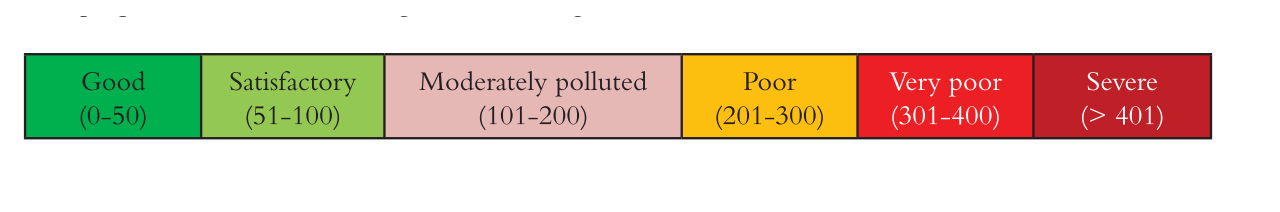
\includegraphics[scale=0.58]{./images/figure13.png}
    \end{center}
   
    \caption{Air Quality Index (AQI) \cite{AirQualityIndex}}
    
    \label{aqi}
\end{figure}


In Canada, the Environmental agency developed AQHI to make the common public aware about the air that surrounds them. It was based on five major pollutants $PM_{2.5}$, $O_3$, $NO_2$, $SO_2,$ and $CO$ initially and later the last two pollutants were dropped from the calculation as they were identified to  contribute very less in predicting health effects. AQHI computed using the following formula.


\begin{equation}
AQHI = \lceil (\frac{1000}{10.4}) \times [e^A-1]+[e^B-1]+[e^C-1] \rceil
\end{equation}

where $ A = 0.000537 \times$ concentration of  $O_3$, $B = 0.000871 \times$ concentration  of $NO_2$ and  $C = 0.000487 \times$ concentration of $PM_{2.5}$.
The value of AQHI varies from 1 to 10+ as shown in figure \ref{aqhi}


\begin{figure}[h]
    \begin{center}
    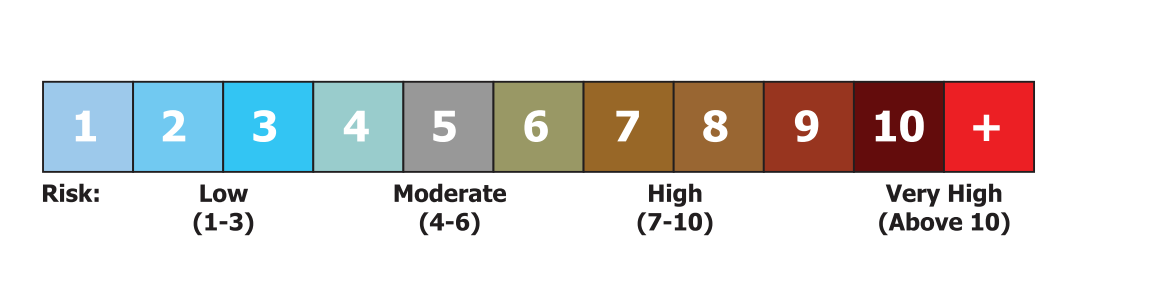
\includegraphics[scale=0.58]{./images/figure12.png}
    \end{center}
   
    \caption{Air Quality Health Index (AQHI) \cite{healthcanada}}
    
    \label{aqhi}
\end{figure}

Now the question is which is a better measure, AQI or AQHI? Health index was created with a different objective which is to provide a combined effects of pollutants to the human health. AQI is based on a single pollutant and hence it is hard to see its direct relationship with health compared to AQHI \cite{Chen2013}. On the other hand AQHI is based on the  the exposure-response relationship between the major air pollutant mix and human health \cite{Chen2013}, which gives more close relation to the mixture of air pollutant than AQI. It is to be noted that both the indices failed to project the health outcomes associated with the exposure to the polluted environment.



\section{Impact of Air Pollution}

Air pollution has significantly increased after the industrialization and urbanization have taken place. The burning of fossil fuels, exhaust from factories and industries, and mining operations are the major contributors to air pollution. The exposure to air pollutants causes premature deaths, cardiovascular disease, stroke, and other respiratory diseases. The state of global air 2017 has discussed the effects of long-term exposure to harmful air pollutants such as particulate matter which contributes to over 4 million premature deaths and is estimated to
double by 2050 if the issue remains unattended \cite{HealthEffectsInstitute2017}. Among the risk factors with the serious health issues, air pollution ranks the highest annually accounting for majority of deaths. The major impacts of air pollution are premature deaths, cardiovascular disease, stroke and other respiratory diseases.
Particles with a diameter of less than 10 microns ($PM10$), and less than 2.5 microns ($PM2.5$) causes the greatest threat to health, as they are capable of penetrating to lungs which leads to cardiovascular and chronic obstructive pulmonary diseases (COPD). \cite{who} \cite{Tian2016}. Exposure to carbon monoxide ($CO$) which is a colorless and odorless gas is absorbed into bloodstream from lungs and reduces the ability to transfer oxygen which inturn affects the functionality of organs such as brain and heart \cite{Sierra-vargas2012} \cite{Golbabaei2012}. Respiratory issues such as decrease in responsiveness of airways, inflammation in airways, lung infectivity occurs due to exposure of high concentration of ozone ($O3$) \cite{Lippmann1989}. Another pollutant is nitrogen dioxide ($NO2$) which causes such as wheezing, coughing, bronchitis and flu. The exposure of mixed air pollutants leads to diverse health effects like birth defects, development delays in children, skin irritation or even cancer \cite{MarilenaKampa2007}.

\section{Background}

The quality of the air has declined since the industrialization has taken place in the mid 19th century. Ever since then it has affected not just the environment but also the human health. There was a development of heavy industries across Europe to North America which used coal as their major source of energy that contributed to black smoke pollution \cite{Heidorn1978} \cite{Timothy}. Coal was not just used in industries but also in houses for heating in winter which made the pollution even worse \cite{Al2016}. These emissions resulted in serious health impacts on residents in urban areas that increased the mortality rate during this period. One such important event in the history of pollution is the great smog of London which killed as many as 12,000 people to death mostly infants. This was caused due to the combination of cold weather with smoke and lasted for several days \cite{londonfog}. There were a string of similar events reported in New York, England, Britain around the same time. All these incidents led to the development of Environmental Protection Agency (EPA) who enforced the need for installing the monitoring stations. The government along with these environmental agencies established acts like clean air act, motor vehicle air pollution act, air pollution control acts for a better quality of air\cite{airpollutionact}. Apart from that they took initiative to monitor the air pollution by installing systems which could measure the concentration of pollutants and could give warnings to public as well as industries regarding the  polluted atmosphere.


\subsection{Existing Environmental Monitoring station}

The government and the Environmental agencies are taking an effort for installing monitoring stations for improving the air quality. The EPA monitors the criteria pollutants along with any special pollutant dominant in that particular area. At present there are two main methods for pollutant measurement: 1) passive sampling, and 2) active sampling \cite{Balakrishnan2015} \cite{activepassive}. These sampling techniques are considered as one of the most significant development for air quality measurement. These approaches are used widely for monitoring purpose. In passive sampling the pollutants are collected by physical process such as diffusion through a static air layer or membrane. pollutants contaminated in the air is diffused to adsorb on the sampling media.

\subsection{Sensor Network for Air Quality Monitoring}







\section{Motivation}

One of the important components in solving this issue is to increase the awareness among public about the current situation and its impact so that they can act on it. The conventional method of monitoring the air quality with the help of a few heavyweight expensive stationary monitoring systems typically installed by the state may not be effective enough for this task. To achieve the goal effectively and without further delay, pollution monitoring must become part of daily activity for everyone. For that the devices to monitor pollution must be small, portable, inexpensive, and part of a global system. With the technological advancement of low cost computing, communication, and sensing devices, and the revolution and the importance of open source software \cite{Anthes2016}, we believe it is possible to build pervasive air pollution monitoring system with commodity hardware and open source software. Now the question is how to design such pollution monitoring devices faster and make them accessible to as many as possible. 
\\
Achieving the above stated goal requires a suitable system framework that can help to accelerate the process of the design and implementation of a air pollution monitoring system using the off-the-shelf commodity hardware and open source software. There are some recent attempts in this direction, but none is comprehensive and simple enough to follow and build a air pollution monitoring system with a little or moderate effort. This thesis is an attempt to fill that gap by first proposing a simple and comprehensive framework and then demonstrating its feasibility and use by creating our own pollution monitoring system that is operational in our lab. We have also added a step of calibration by implementing a web-based tool to find out the quality of data obtained from the system. Our contribution is a step towards inspiring and motivating not only the public to use the device, but also many amateur electronic hobbyists to buy the hardware locally and download the associated software to build their own pollution monitoring device.


\section{Research Problem}
The aim is to design and develop an air pollution monitoring system using off the shelf
hardware and open source software and analyze the quality of data obtained through calibration with the following objectives in mind.
\begin{enumerate}
    \item To develop a calibration tool which could give how accurate the sensor data is when compared with referance data.
    
    \item To educate the common people on adverse effect of air pollution by showing how polluted
    the vicinity is.
    
    \item To influence the behaviour of people by representing the concentration of pollutant as well
    as AQHI (Air Quality Health Index) which provides the seriousness that pollutants cause
    to health.
    
    \item To give an idea of how to integrate all the hardware components to a processor and also
    make an independent software, which can be accessed anywhere in the world.
    
    \item To encourage and help citizen science to solve the issue of air pollution and give more
    understanding to the impact it cause to human health and environment.

\end{enumerate}


\section{Thesis Contribution}


\section{Research Question}
 
 Some important research questions to be addressed related to the issue of air quality are: 

 \begin{enumerate}
  \item What kind pollutants affect the human health most? How to measure them?
   
  \item  As the pollution is in the atmosphere, should it not be measured everywhere all the time? If so, what kind of infrastructure is needed to facilitate such a ubiquitous measurement?
  
 \item What all factors should be considered while selecting sensors for measurement of pollutants?
 
 \begin{enumerate}
 \item Accuracy of the data collected from the sensors.
 \item The cost of the sensors.
 \item The size of the sensors.
 \item Integration with the processor.
 \end{enumerate}

 \item Which processor to be used for processing the data collected from sensors?
 
 \begin{enumerate}
 \item The ability to process analog signals collected from the sensor.
 \item Opens source platform.
 \item Ability to use in real time application.
 \item Able to connect with the Wi-Fi module easily.
 \end{enumerate}

 \item How should the hardware component i.e the sensors and the processor, should be packaged?
 
 \begin{enumerate}
\item As compact as possible.
\item The value of the sensors should not be affected.  
 \end{enumerate}
 
 
   \item What is the difference between different metrics which is used to show       	the effect of pollution?
   \begin{enumerate}
   \item Understanding why different indexes are used for pollution monitoring.
   \item To identify which all indexes should be displayed in the software.
   \item Out of all the indexes which one is the most relevant to public and why?
  
   \end{enumerate}
  
 \item How can the seriousness of pollution be made aware?
 \begin{enumerate}
 \item What all graphs or charts to be used?
 \item How to make a impressive software tool for demonstration?
 \end{enumerate}
 
 \item How can the representation of Air quality metrics be done?
\begin{enumerate}
\item Should there be any categorization within the society for data visualization?
\item If so, what all data should be shown for each section?
\item How to demonstrate a simple view of complex effectively?
\end{enumerate}
 
 

 
 \end{enumerate}
 
\section{Research Challenges}


The major challenges expected on creating a complete system are:

\begin{enumerate}


\item The integration of different sensors with the processor.
\par
As each sensors are having its own properties, there can be a issue when connecting all of them together in a single platform. Most of the sensors used for measurement are heat sensor and needs to be powered atleast 12 hours before operating. There is a particular operating temperature range for each sensors connected. As each of the sensor needs different environment for working, all the factors should be incorporated for a complete working environment.

\item Integration of communication module which is  WiFi with processor as this module alone requires a different voltage level to drive.
\par
The data transferring module used here is a WiFi module which needs a separate voltage level of 3.3 Volt when compared to the sensors which are driven with a voltage of 5 Volt each. On giving any voltage more than 3, will burn the entire module and hence it needs a separate voltage line to be given. 

\item Calibration of each sensors based on the data sheet.
\par
As I am selecting commodity sensors which says that it is already calibrated but usually it should be done for each environment. The data collected changes for each environment and this should be taken care of. This can be a tough task as for each of the sensors it changes based on the slope of internal resistance and the internal voltage values given in data sheet. 
\item Packaging of hardware component.
\par
To make the whole system portable it should be packed carefully. For certain sensor like dust sensor, it should be exposed to the environment so as to get the value of particulate matter. This packing should be done in such a way that the it does not hinder with the observed value.

\item Transferring the data to a platform or a database using the WiFi module.

\item Checking whether the collected data is accurate.


\end{enumerate}

\section{Structure of the Thesis}